\documentclass[grey,handout]{beamer}
%\usetheme{Pittsburgh}
\usetheme{Montpellier}
\usepackage{amsmath}
\usepackage{graphicx}
\usepackage{multicol}

\renewcommand{\frametitle}[1]{\begin{center}\textbf{#1}\end{center}}

\def\dd{{\rm d}}
\def\E{\mathbb{E}}
\def\BigO{{\cal O}}

\begin{document}
\title{Numerical Comparative Dynamics: Ball Python Breeding}

\author{Donald M.~DiJacklin}
\date{23 July 2018}

\begin{frame}
  \titlepage
\end{frame}

\begin{frame}
\frametitle{ROADMAP OF SEMINAR}
  \begin{enumerate}[<+->]
    \item Goal
    \item Truths
    \item Assumptions
    \item Data
    \item Theory
    \item Results Thus Far
  \end{enumerate}
\end{frame}
\begin{frame}
\frametitle{Goal}
To find the effects changing parameters have on a Ball Python Breeding Program.
\end{frame}
\begin{frame}
\frametitle{Truths}
  \begin{enumerate}[<+->]
    \item Males can inseminate 5 females apiece.
    \item About 60\% of pairings result in a `clutch'.
    \item It costs about \$80 to keep a snake for a year.
    \item A male takes a year to grow to a breedable size.
    \item A female takes two years.
  \end{enumerate}
\end{frame}
\begin{frame}
  \frametitle{Assumptions}
  \begin{enumerate}
    \item Clutch size is distributed discrete triangular [3,14] max 6.
    \item A breeder has a capacity that they are not willing to exceed.
    \item No sickness.
  \end{enumerate}
\end{frame}
\begin{frame}
\frametitle{Data}
I went to Repticon in Tampa and recorded the price, sex, and traits of each snake. I recorded these in a csv and then filtered out genes that had fewer than 10 traits represented, and the snakes that had them.
\end{frame}
\begin{frame}
  \frametitle{Theory}
\end{frame}
  \begin{frame}
  \frametitle{Tweak of Becker 1973}
  Supposing you start with $I$ males and $J$ females, and $I+J$  is less than your total capacity.
  \begin{align*}
    \max_\Pi&\left\{ \sum_{t=1}^{\infty}\sum_{i\in I_t}g\left(m_i,f_{\Pi(i)},t\right)\delta^t \right\}\\
    s.t. &\quad I_t+J_t\leq C
  \end{align*}
  where $\Pi$ maps to possible subsets of 5 or less elements of the set of females $J_t$, and $C$ is the capacity.
\end{frame}
\begin{frame}
  \frametitle{Problems}
  \begin{itemize}
    \item Not PAM or NAM.
    \item $g$ may be a profit function, but there doesn't seem to be a closed form for $\Pi$
    
    \item Brute force method is $\BigO(IJ^4)$ in each period.
  \end{itemize}
\end{frame}
  \begin{frame}
  \frametitle{Approximations}
  \end{frame}

  \begin{frame}
    \frametitle{Maximize Average Profits}
    \begin{align*}
      \max_{\mathbf{X},\mathbf{y},\mathbf{z}}&\left\{ \sum_{i\in I}\mathbf r_i \mathbf x_i^T - 80\mathbf y^T\mathbf 1_I - 80\mathbf z^T\mathbf 1_J \right\}\\
      s.t. & \quad\mathbf X\mathbf 1_J \leq 5\mathbf 1_I \\
      &\quad \mathbf X^T \mathbf 1_I \leq \mathbf1_J\\
      &\quad \mathbf X \mathbf1_J\leq M\mathbf y\\
      & \quad\mathbf X^T\mathbf 1_I \leq M\mathbf z\\
      &\quad \mathbf y^T\mathbf 1_I + \mathbf z^T\mathbf 1_J \leq 15\\
      & \quad X_{ij}, y_i, z_j \in \{0,1\}
    \end{align*}
  \end{frame}
\begin{frame}
    \frametitle{Maximize Weighted Number of Genes}
    This is what snake breeders actually do, and I implemented it as follows:
    \begin{align*}
    \max_{\mathbf{X},\mathbf{y},\mathbf{z}}&\left\{ \sum_{i\in I} \mathbf g_i \mathbf x_i^T  \right\}\\
      s.t. & \quad\mathbf X\mathbf 1_J \leq 5\mathbf 1_I \\
      &\quad \mathbf X^T \mathbf 1_I \leq \mathbf1_J\\
      &\quad \mathbf X \mathbf1_J\leq M\mathbf y\\
      & \quad\mathbf X^T\mathbf 1_I \leq M\mathbf z\\
      &\quad \mathbf y^T\mathbf 1_I + \mathbf z^T\mathbf 1_J \leq 15\\
      & \quad X_{ij}, y_i, z_j \in \{0,1\}
    \end{align*}
\end{frame}

\begin{frame}
\frametitle{Results Thus Far}
\end{frame}

\begin{frame}
\frametitle{Show my decision rule is better}
  \begin{multicols}{2}
  \begin{figure}[H]
  \centering
  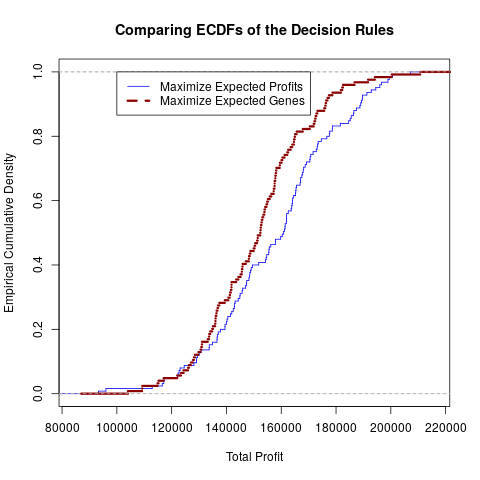
\includegraphics[width=.5\textwidth]{ECDF.png}
  \end{figure}
  \begin{figure}[H]
  \centering
  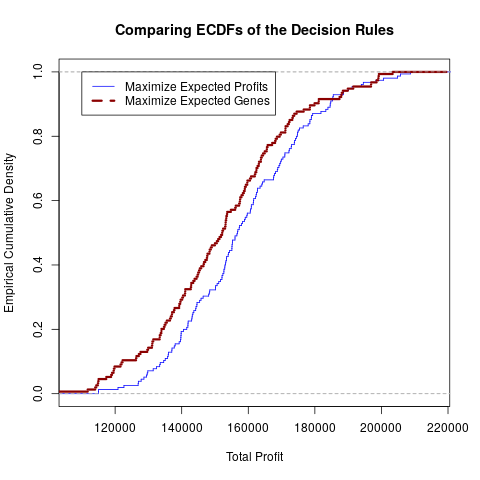
\includegraphics[width=.5\textwidth]{newECDF.png}
  \end{figure}
  \end{multicols}
  151096.2  152198.7  157535.2
\end{frame}

\begin{frame}
  \frametitle{Probability of Clutch}
  \begin{figure}[H]
  \centering
  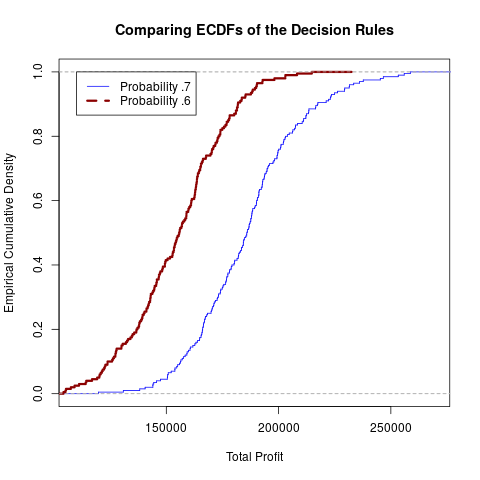
\includegraphics[width=.5\textwidth]{probECDF.png}
  \end{figure}
  157535.2  186213
\end{frame}

\begin{frame}
  \frametitle{Distribution}
  \begin{multicols}{3}
  \begin{figure}[H]
  \centering
  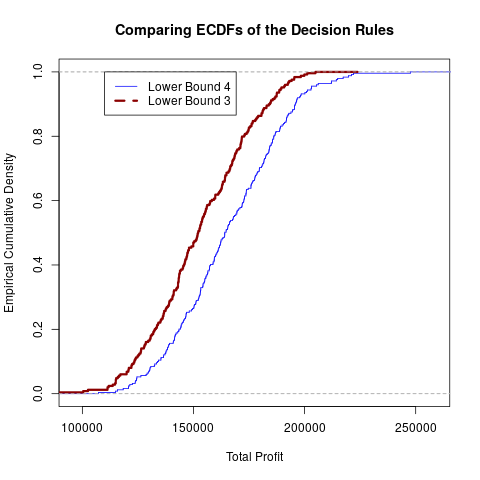
\includegraphics[width=.3\textwidth]{lbECDF.png}
  \end{figure}
  \begin{figure}[H]
  \centering
  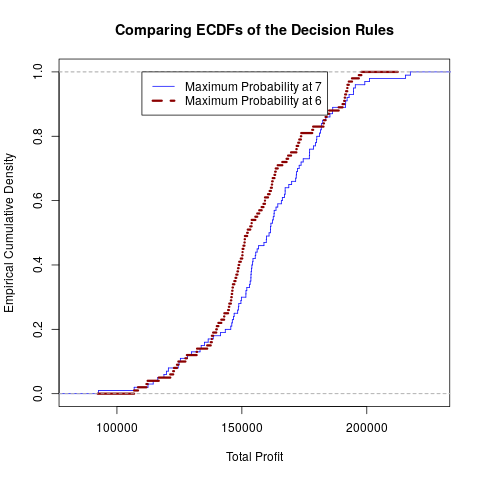
\includegraphics[width=.3\textwidth]{maxECDF.png}
  \end{figure}
  \begin{figure}[H]
  \centering
  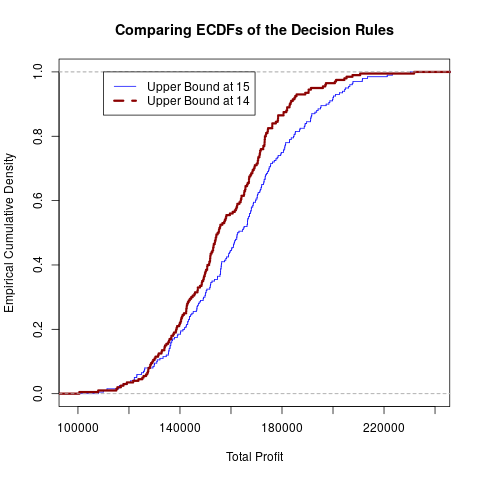
\includegraphics[width=.3\textwidth]{ubECDF.png}
  \end{figure}
  
  \end{multicols}
\end{frame}


\begin{frame}
  \frametitle{Capacity}
  \begin{multicols}{2}
  \begin{figure}[H]
  \centering
  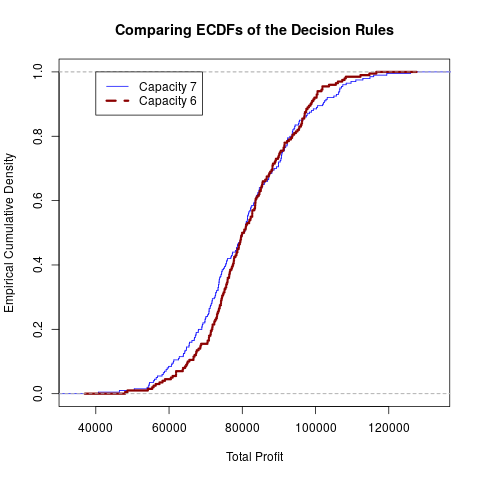
\includegraphics[width=.5\textwidth]{capECDF.png}
  \end{figure}
  80799.23 81569.97
  \begin{figure}[H]
  \centering
  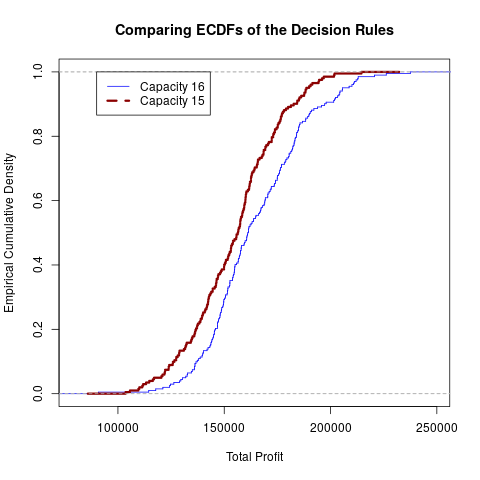
\includegraphics[width=.5\textwidth]{othcapECDF.png}
  \end{figure}
  154631.8 164730.1
  
  \end{multicols}
  
  
  \end{frame}

\end{document}